%%% template.tex
%%%
%%% This LaTeX source document can be used as the basis for your technical
%%% paper or abstract. Intentionally stripped of annotation, the parameters
%%% and commands should be adjusted for your particular paper � title, 
%%% author, article DOI, etc.
%%% The accompanying ``template.annotated.tex'' provides copious annotation
%%% for the commands and parameters found in the source document. (The code
%%% is identical in ``template.tex'' and ``template.annotated.tex.'')

\documentclass[annual]{acmsiggraph}
\usepackage{amsfonts}
\usepackage{algorithm}
\usepackage{algorithmic}
\usepackage{graphicx}
\TOGonlineid{45678}
\TOGvolume{0}
\TOGnumber{0}
\TOGarticleDOI{1111111.2222222}
\TOGprojectURL{}
\TOGvideoURL{}
\TOGdataURL{}
\TOGcodeURL{}

\title{CS5643 Final Project Report: \\ Modeling Seed Dispersal via Fluid Simulation with Rigid Body Coupling}

\author{Michael Flashman\thanks{e-mail:mtf53@cornell.edu}\\Cornell University \and Tianhe Zhang \thanks{e-mail:tz249@cornell.edu}\\Cornell University}

\pdfauthor{Michael Flashman, Tianhe Zhang}

\keywords{simulation, rigid fluid, plant seeds, wind dispersion}

\begin{document}

\maketitle

\begin{abstract}
Wind dispersal of  seeds is an important mechanism of mobility in many plant species.  Unlike other seed dispersal mechanisms , wind dispersal is chiefly a function of seed morphology.  Primarily isolated from the  complex ecology of the plant's environment during this critical stage of a life, physical simulation provides a way to  quantify the fitness of different seed morphologies .   As a first step toward this quantification, we  implement a  framework for stable 2D fluid simulation with  coupling to radially parametrized rigid bodies via the stable fluid method.   We demonstrate that these simulation methods are capable of generating plausible flight behavior such as fluttering and tumbling, critical to 2D dispersion.   Using this framework we perform random sampling of different shapes to obtain preliminary data on the distribution of various flight characteristics. 	 
\end{abstract}

\keywordlist


\section{Biological Overview }
(Note: This biological overview is adapted from the one given in our original project proposal, and is included only for completeness. )
\\ 
\\
Dispersion is the process by which an organism moves away from its place of birth.  This process is central to understanding  population structure and dynamics, gene-flow, evolution and speciation, as well as many other biological phenomena \cite{levin1989}.   In general, the mechanism for dispersion is difficult to model precisely. An organism may be mobile for its entire life, and its motions may be dictated by complicated behavior and interactions with other species.  For sessile organisms, the dispersal process is often restricted to a single phase in the organism's life in which the organism is essentially passive \cite{nathan2000}.   Such organisms lend themselves to more precise understanding of the dispersal process.  

Seed plants serve as a model species for studying dispersal. Even as a passive agent, the mechanisms behind seed dispersal can be surpassingly complex \cite{wilson2000}.  Fruits, which beer a seed at their center, are dispersed by frugivors, typically as a result of being eaten and later expelled with the fecal matter.  While the seed remains passive, the dispersal process is strongly coupled  to the complex behavior of the carrier, making precise modeling difficult.   In contrast, wind dispersal is an entirely physical process, predominately decoupled from complex biological interactions.    

Wind dispersed seeds have been studied previously through empirical analysis of seed morphology and flight characteristics \cite{augspurger1986}.  This work has been applied to  theoretical ballistic and plum models  to obtain plausible explanations for spatial population dynamics and pattern formation \cite{levin2003}. Recent work has also considered  evolutionary implications of spatial segregation of  plant species as a result of wind dispersal by looking at phenotypic changes across  populations \cite{Cheptou2008}.   A theoretical investigation of dispersal driven speciation is carried out in \cite{levin2010}. 

This research together  describes a closed cycle in a biological story: seed morphology determines  dispersal, dispersal determines spatial population dynamics, spatial population dynamics determine genetic mixing, and genetic mixing determines new seed morphology.\footnote{In reality, this simple story of dispersion driven evolution is complicated by several factors. Seed morphology  plays an important  role in  other stages in a plant's life cycle. Seed size, for instance, influences germination success rate.  Inter-species competition effects  the evolution of plant characteristics.   Though seed morphology may not be effected directly, parameters coupled to dispersal, such as plant height and population density will be.  Finally, seed fitness is measured not by dispersive capacity, but by maximizing the likelihood that  seeds land in suitable habitat for germination.  But the distribution of suitable habitats is strongly affected population level competition. }  

Understanding how phenotypic changes to seed shape affect  flight characteristics remain a difficult but important challenge to the field, providing a link between phenotypic variation and dispersive outcome.  Some success has been achieved by construction low-dimensional flight models based on classical aerodynamic theory \cite{greene2005}.  However, careful physical modeling and simulation reveals that natural structures exhibit behavior that is not accurately described by aerodynamic theory, and instead depends on a full consideration of fluid and rigid-body coupling \cite{wang2005}\cite{wang2012}.   Given the tremendous increase in computing power and speed,  precise physical simulation is a viable approach to the problem.

One of the most interesting features of a simulation based approach to understanding seed dispersion is that it allows us to consider seed shapes not observed in nature.  This freedom allows us to consider a number of problems that would  otherwise be  difficult to approach.  For instance, by looking at flight characteristics of seed shapes similar to those observed in nature, we can asses local stability and optimality of reel seeds.

Further, we may sample the space of all possible seed morphologies to generate a complete map of flight characteristics.  In this way, we can generate a complete fitness landscape of seed morphology.\footnote{In reality, the fitness landscape for wind dispersed seeds is measured not only by how far a seed travels, but also by how often a seed falls in a habitable zone.  The distance plays an important role in the long term survival of the species, but the later is necessary for successful germination.}   While such a perspective is out of reach for most biological phenomena, the distinctly physical nature of wind based seed dispersion provides a unique glimpse into the diverse space of possible morphologies and the evolutionary pathways that connect them.   

Given this project's relative infancy, we do not consider the research agenda described above in all it's glory, but instead focus instead on the simplified case of 2D dispersion of elliptic shapes.  Even in this simplified version of the problem, we observe subtle variations in shape and behavior.  This experiment and preliminary results are discussed further in Section 3.  



\section{Technical Description}

\subsection{Fluid (Smoke)}
Our fluid simulation implementation is based on the source code provided for smoke simulation and control. Though not entirely relevant to our  goal of modeling seed dispersion, we began by implementing various features of the smoke control project.  Following  \cite{fattal2004}, we introduce a gathering force $G$ to make the smoke converged to a given keyframe density:
$$ \mathbf{G}(\mathbf{\rho}, \mathbf{\rho}^*)  = \nabla \cdot [\mathbf{\rho} \tilde{\mathbf{\rho}}^* \nabla(\mathbf{\rho} - \mathbf{\rho}^*)]$$
where $\bf{\rho}^*$ is the keyframe smoke density and $\tilde \bf{\rho}^*$ is the keyframe smoke density blurred to better match the diffusive quality of the simulated smoke.

The smoke simulation is subject to significant numerical dissipation.  To eliminate this undesirable affect, we impose a simple normalization condition to maintain the density sum equal to the sum of keyframe density.  Specifically,  we require that the total mass of smoke  in the scene is equal to the total mass of smoke density in the keyframe.  If not, we scale our original density until the target density mass is met:
	$$\rho_{ij} = \rho_{ij}\left [ 1 +  \alpha \sum (\rho_{ij}^* - \rho_{ij} ) / N^2 \right] \text{ with } \alpha \in [0,1] $$
In practice we use the modified normalization expression :
	$$\rho_{ij} = \rho_{ij}\left[ 1  + \alpha  (\rho_{ij}^* - \rho_{ij} ) \right ] \text{ with } \alpha \in [0,1] $$
which actively destroys smoke density not matching the key frame.  We find that this destructive feature to nicely manage the spatial numerical dissipation. 

For simplicity, our simulation runs on a good old-fashioned $N\times N$ lattice.  To improve numerical accuracy, we employ a sudo-MAC grid approach to calculate derivatives at cell boundaries (rather than across neighboring lattice points) as need.  That is, we compute derivatives that we would usually associate with the secondary grid of the MAC grid.  


\subsection{Rigid Body Coupling}
We implement rigid body coupling to our fluid simulation using the rigid fluid method described in \cite{carlson2004}. In this approach, each rigid body is treated as a fluid with body specific density.  After the fluid equations are solved, the updated fluid is used to determine the update to the rigid-body, and finally rigidity condition is imposed on the fluid  from the rigid body.

According to equation (17) in the paper, the forces that arises from the relative density of the  can be expressed as 
$$ \mathbf{S} = \rho_r \mathbf{A}_c + \mathbf{r}_i \times \rho_r \alpha_c - (\rho_r - \rho_f) [\frac{\mathbf{u}^* - \mathbf{u}^n}{\Delta t} + (\mathbf{u}^* \cdot \nabla )\mathbf{u}^* - \mathbf{f}]$$
Since we are only interested in isolated rigid bodies, we do not consider rigid-body rigid-body collisions  in our system. Then $\mathbf{S}$  becomes
$$ \mathbf{S}' = - (\rho_r - \rho_f) [\frac{\mathbf{u}^* - \mathbf{u}^n}{\Delta t} + (\mathbf{u}^* \cdot \nabla )\mathbf{u}^* - \mathbf{f}]$$
where $\mathbf{u}^*$ is the velocity of the fluid  after solving the fluid equations  at the current time step but before considering rigid body coupling. $\mathbf{u}^n$ is the velocity from the previous iteration. $\rho_r$ is the density of the rigid body, $\rho_f$ is the density of the fluid, and $\mathbf{f}$ represents any external forces on the system.

%In order to compute the term $(\mathbf{u}^* \cdot \nabla )\mathbf{u}^*$, assume $\mathbf{u}^* = \binom{u}{v}$, then
%\begin{equation}
%\begin{split}
%(\mathbf{u}^* \cdot \nabla )\mathbf{u}^*& = (u \partial_u + v \partial_v)\mathbf{u}^* \\
%& = \binom {u \partial_u u + v \partial_v u}{ u \partial_u v+ v \partial_v v}
%\end{split}
%\end{equation}
%Then we applied the MAC grid to calculate $\partial_u u, \partial_u v, \partial_v u \mbox{ and } \partial_v v$.

Using $\mathbf{S}$ we update a  new velocity field that incorporates rigid body behavior,
$$\hat{\mathbf{u}} = \mathbf{u}^* + \mathit{w}\frac{\Delta t}{\rho_r}\mathbf{S}$$
where $\mathit{w}$ is the fraction of the cell that is part of the rigid body. To obtain this $\mathit{w}$ at the boundary of our rigid body , we used the supersampling technique. 

In order to maintain the rigidity, we need to obtain $\hat{\mathbf{v}}_i$ and $\hat{\omega}_i$ for each rigid body. We calculate them by integrating $\hat{\mathbf{u}}$ inside a given rigid body $\mathbb{R}_i$ with the following equations:
$$ M_i \hat{\mathbf{v}}_i = \int_{\mathbb{R}_i} \rho_i \hat{\mathbf{u}} dg_i$$
$$ \mathbf{I}_i \hat{\omega}_i = \int_{\mathbb{R}_i} \mathbf{r}_i \times \rho_i \hat{\mathbf{u}} dg_i$$
where, $dg_i$ is the column of the cell occupied by the solid (can be calculated by $\mathit{w}$).
Then, we can find $\hat{\mathbf{u}}_R$ by
$$ \hat{\mathbf{u}}_R = \cup_i (\hat{\mathbf{v}}_i + \hat{\omega}_i \times \mathbf{r}_i) $$
and get our final velocity:
$$\mathbf{u}^{n+1} = (1-\mathit{w})\hat{\mathbf{u}} + \mathit{w}\hat{\mathbf{u}}_R$$
 
In our implementation, we go through each cell in the grid two times. The first time, we find out $\hat{\mathbf{v}}_i$ and $\hat{\omega}_i$ by cumulating $\rho_i \hat{\mathbf{u}} dg_i$ and $\mathbf{r}_i \times \rho_i \hat{\mathbf{u}} dg_i$ at each cell. The second time, we use the calculated $\hat{\mathbf{v}}_i$ and $\hat{\omega}_i$ to compute $ \hat{\mathbf{u}}_R $ and to update the new velocity $\mathbf{u}^{n+1}$ .

\subsection{Stable Solver}
The provided base code comes complete with a simple Gauss-Seidel iterative linear solver. To improve the performance of the fluid solver, we implemented the Preconditioned Conjugate Gradient (PCG) linear solver. Pseudo code for this method is provide in Algorithm \ref{alg1}  \cite{kincaid2002}.  In the interest of time we use the simplest  pre--conditioner:  $Q = \text{diag}(M)$.  At present, this pre--conditioner yields  marginal improvements over the provided .  Preconditioning with something like the Incomplete Cholesky factorization of A would be preferable.  

\begin{algorithm}
\caption{Preconditioned Conjugate gradient algorithm }
\label{alg1}
\begin{algorithmic}
\STATE \textbf{input} $x$, $A$, $b$, $Q$, $\delta$, $\varepsilon$
\STATE $r\leftarrow b - Ax$
\STATE solve $Qz = r$ for $z$
\STATE $v \leftarrow z$
\STATE $c \leftarrow \langle z, r \rangle$
\FOR{ $k =1$ \textbf{to} $M$ do}
	\IF {$\langle v, v \rangle^{1/2} \le \delta$}
		\STATE exit loop
	\ENDIF
	\STATE $z \leftarrow Av$
	\STATE $t \leftarrow c/\langle v, z \rangle$
	\STATE $x \leftarrow x + tv$
	\STATE $r \leftarrow r - tz$
	\STATE solve $Qz = r$ for $z$
	\STATE $d \leftarrow \langle z, r \rangle$
	\IF {$d \le \varepsilon$}
		\IF {$\langle r, r \rangle \le \varepsilon$}
			\STATE exit loop
		\ENDIF
	\ENDIF
	\STATE $ v \leftarrow z + (d/c)v $
	\STATE $ c \leftarrow d$
	\STATE \textbf{output} k, x, r
\ENDFOR
\end{algorithmic}
\end{algorithm}

\subsection{Rigid Bodies}
Toward the support of arbitrary seed dynamics simulation, we provide general support for  shapes parametrizable by a radial function $r(\theta)$.   The implementation is provided in the \textbf{RigidPolarShape} class. Assuming that \textbf{radialFunction(theta)} is specified in a child class, this class computes basic physical quantities such as total mass, moment of inertia, etc by direct numerical integration.  This class also handles percent cell inclusion computations  ( $w$from Section 2.2). 

Arbitrary shape support is hard, so we are in one sense settling.  At the same time, the space of shapes parametrized by radial function is actually quite general.  In addition it comes with a natural set of basis functions.  By selecting a particular set of principle basis functions, we are well suited to sample the shape space in a principled way.  

\subsection{Colorful Smoke}   
To make our smoke look interesting, we also implemented a colorful smoke. The idea is that instead of just solve the grayscale density, we run the solver three times to solve the RGB densities separately. In order to do that, we changed the \textbf{SmokeKeyframe} function so that it retrieves the RGB data from the target figure. 

\begin{figure}[ht]
\begin{center}
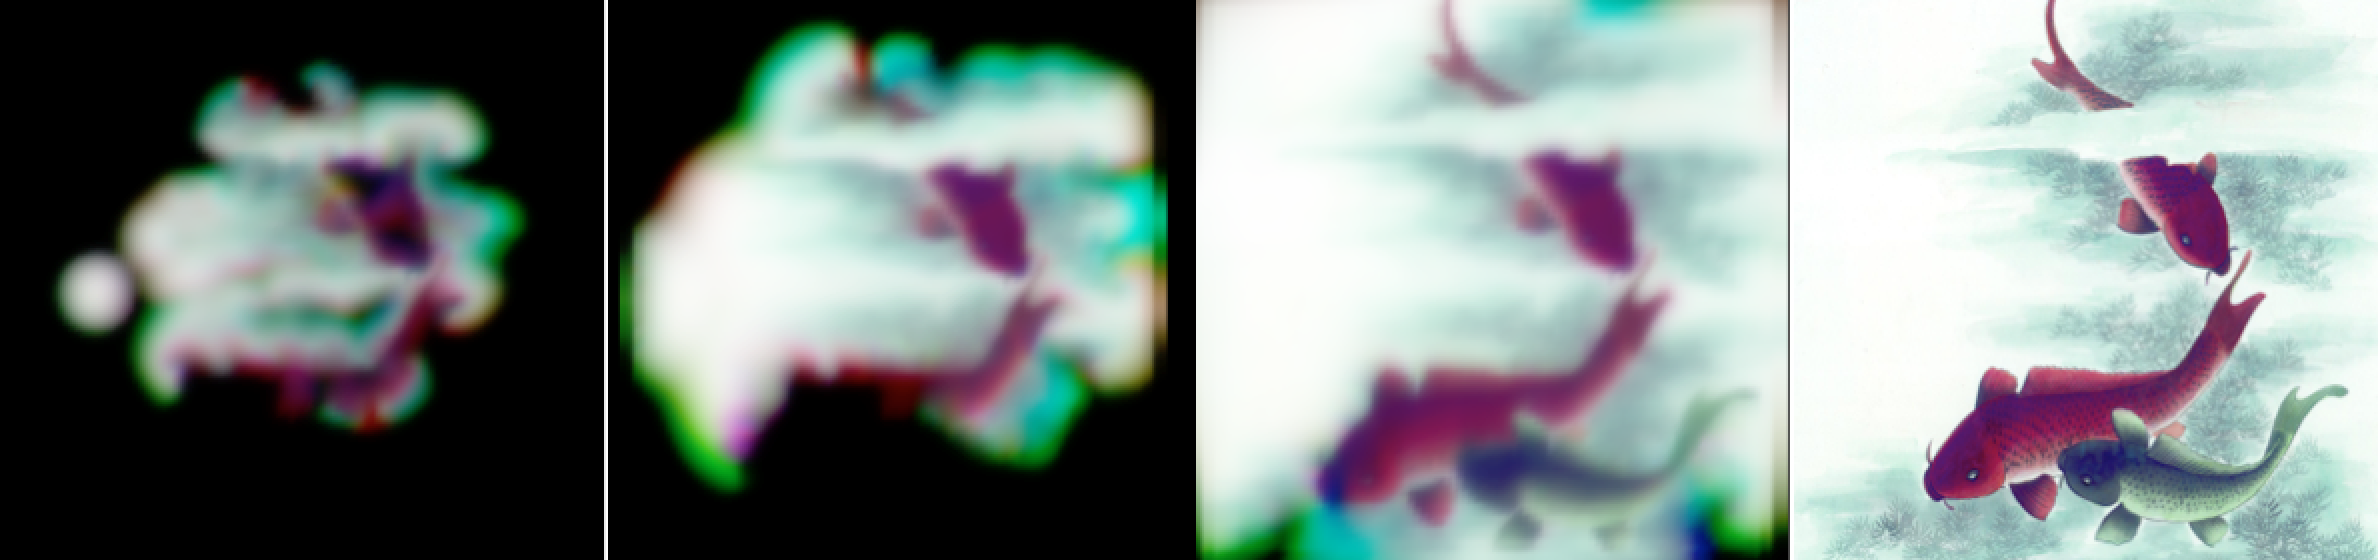
\includegraphics[width=240pt]{fish.png}
\caption{First three photos are take during color smoke animation. The fourth one is the target image. }
\end{center}
\end{figure}

\pagebreak
\section{Experiment and Results}
\subsection{Experiment Setup}
We perform a 2D version of the experiment described at the end of Section 1 using the fluid with rigid body simulation framework described in Section 2.  For this preliminary round of experiments, we focus in particular on elliptic seed shapes which can be easily parametrized by a major axis and a minor axis. The experiment is outlined below:
\begin{enumerate}
\item  Generate a new seed shape by  choosing random major and minor axis.  
\item  Drop the shape several times at different orientations.  We opt to step through a finite number of specific orientation, but random sampling could be performed as well.
\item Measure: average velocity, terminal velocity, average horizontal displacement , max  horizontal displacement, final position, etc.  
\item Repeat experiment from Step 1.
\end{enumerate}  
For more implementation details, please see file \textbf{SeedDrop.java}.

\subsection{Results and Discussion}
In our principle experimental run, we simulated forty different shapes and for each shape, we performed ten drops at relative density 10 (where the fluid density is 1).  Sampling is performed according to :
$$ a = 4 + 4*\text{rand} \;\;\; \text{and} \;\;\; b= 1+ 3*\text{rand} $$
where $a$ is the major axis and $b$ is the minor axis.  Some data from the preliminary trials is saved in the \textbf{Data} directory.  Movies for a few of these trials can be found in the \textbf{Artifacts} directory.  

We will not stress the precise numerical details of the simulation but it is worth observing the two principle modes of behavior demonstrated by the various trials: fluttering and tumbling.    In two dimensions, these are the only modes of falling. And which mode a given shape lies in has dramatic  implications for the particular characteristics of the fall.  For instance, tumbling behavior supports significant horizontal displacement where as fluttering behavior tends to leave the falling shape roughly where it started.  More interesting is that the shapes which exhibit tumbling seem to lie in an intermediate range in the space of ellipses, with eccentricity on the order of 0.5.  

We also provide a few plots of our data in Fig~2 and Fig~3.  As hinted at above, both plots indicate a curious transition point in behavior near eccentricity of 0.5.  The first plot, indicates that  flutter/tumbling is maximal near this critical point. The second plot, depicts an abrupt drop in average velocity at this critical point.   

\section{Conclusion}
We have described a simulation based approach for quantifying the aerodynamics of random 2D shapes.  In the context of plan seed dispersion, this approach provides for an (approximate) global understanding of the fitness landscape for seed morphology.  While we only present preliminary results as  proof of concept, they already  hint at a surprising landscape of behavior across shapes.  It is our hope that  extensions of this  approach will provide new understanding of seed morphology, dispersal, population dynamics, and evolution.

\nocite{*}
\bibliographystyle{acmsiggraph}
\bibliography{bibliography}

\begin{figure*}
\begin{center}
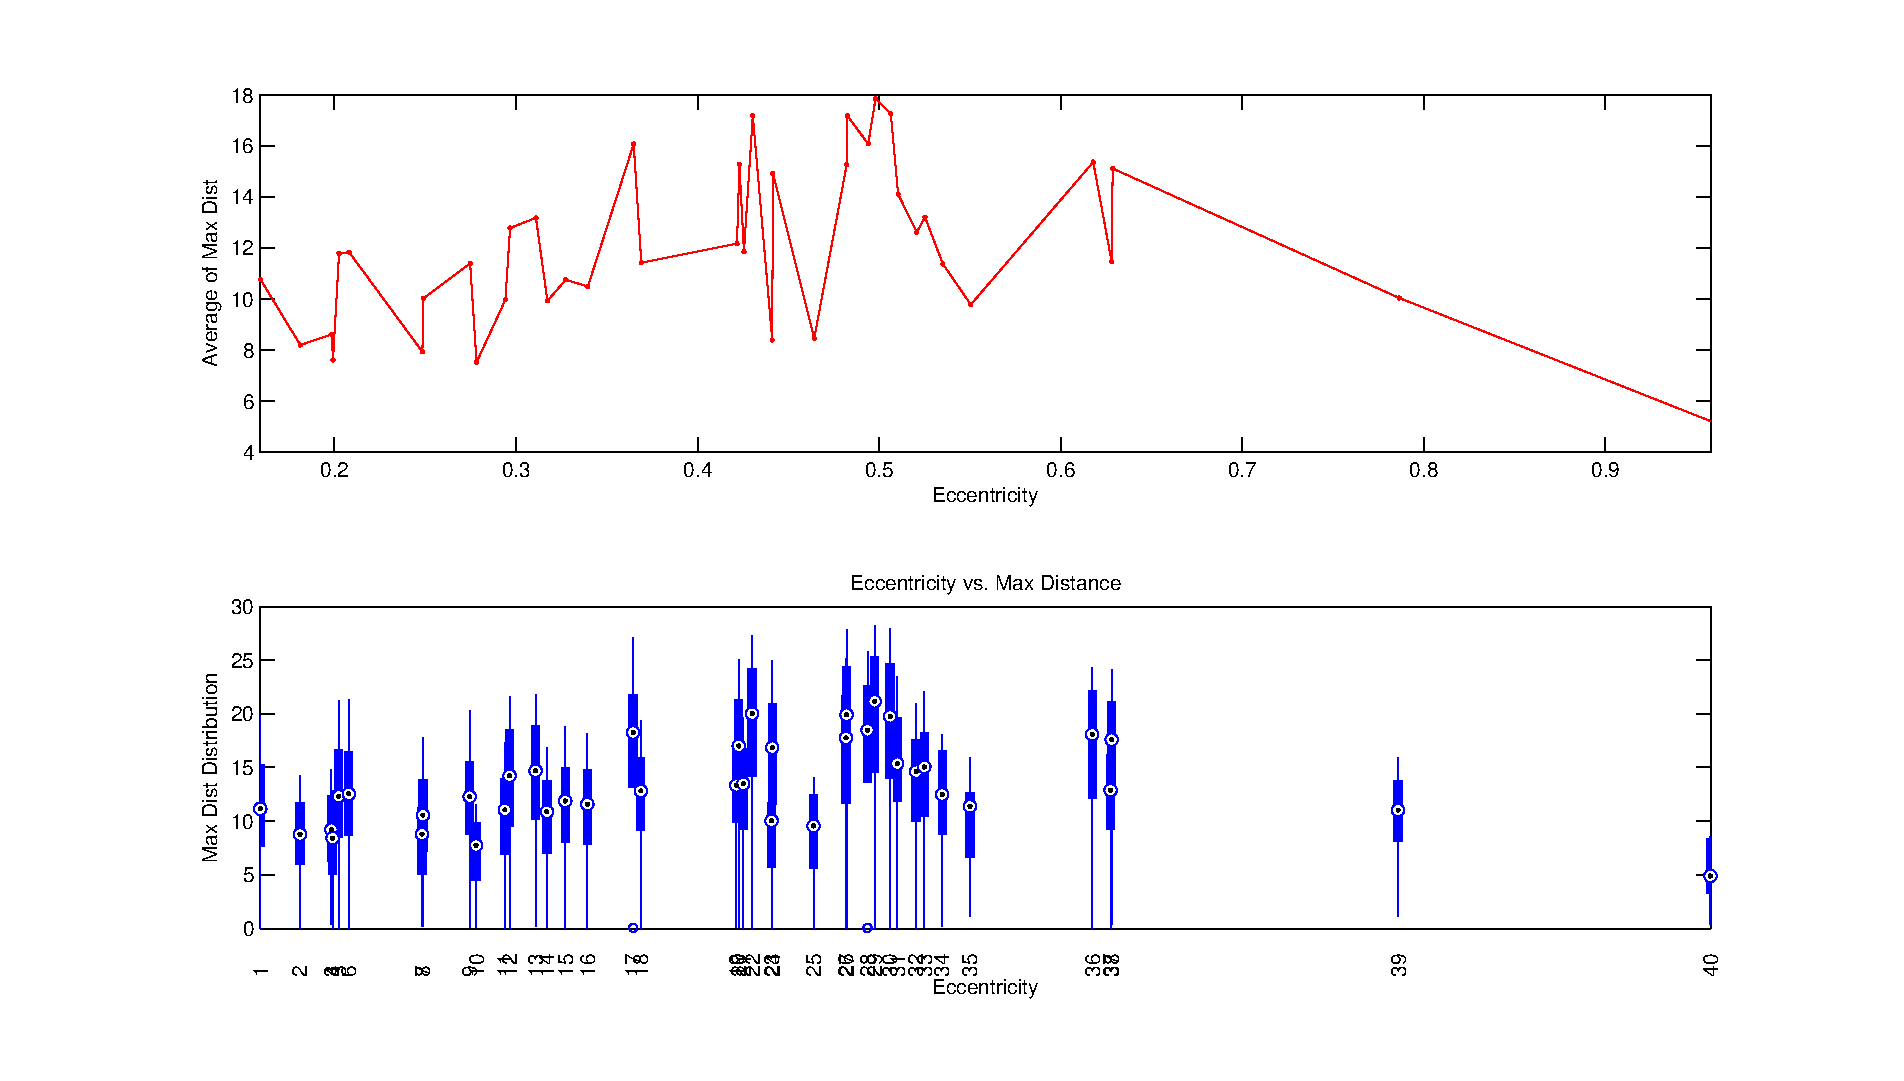
\includegraphics[width=500pt]{fig1.eps}
\caption{Ellipse eccentricity vs maximum horizontal displacement.  y-values were obtained by averaging over the multiple drops for each shape.  }
\end{center}
\end{figure*}
 

\begin{figure*}
\begin{center}
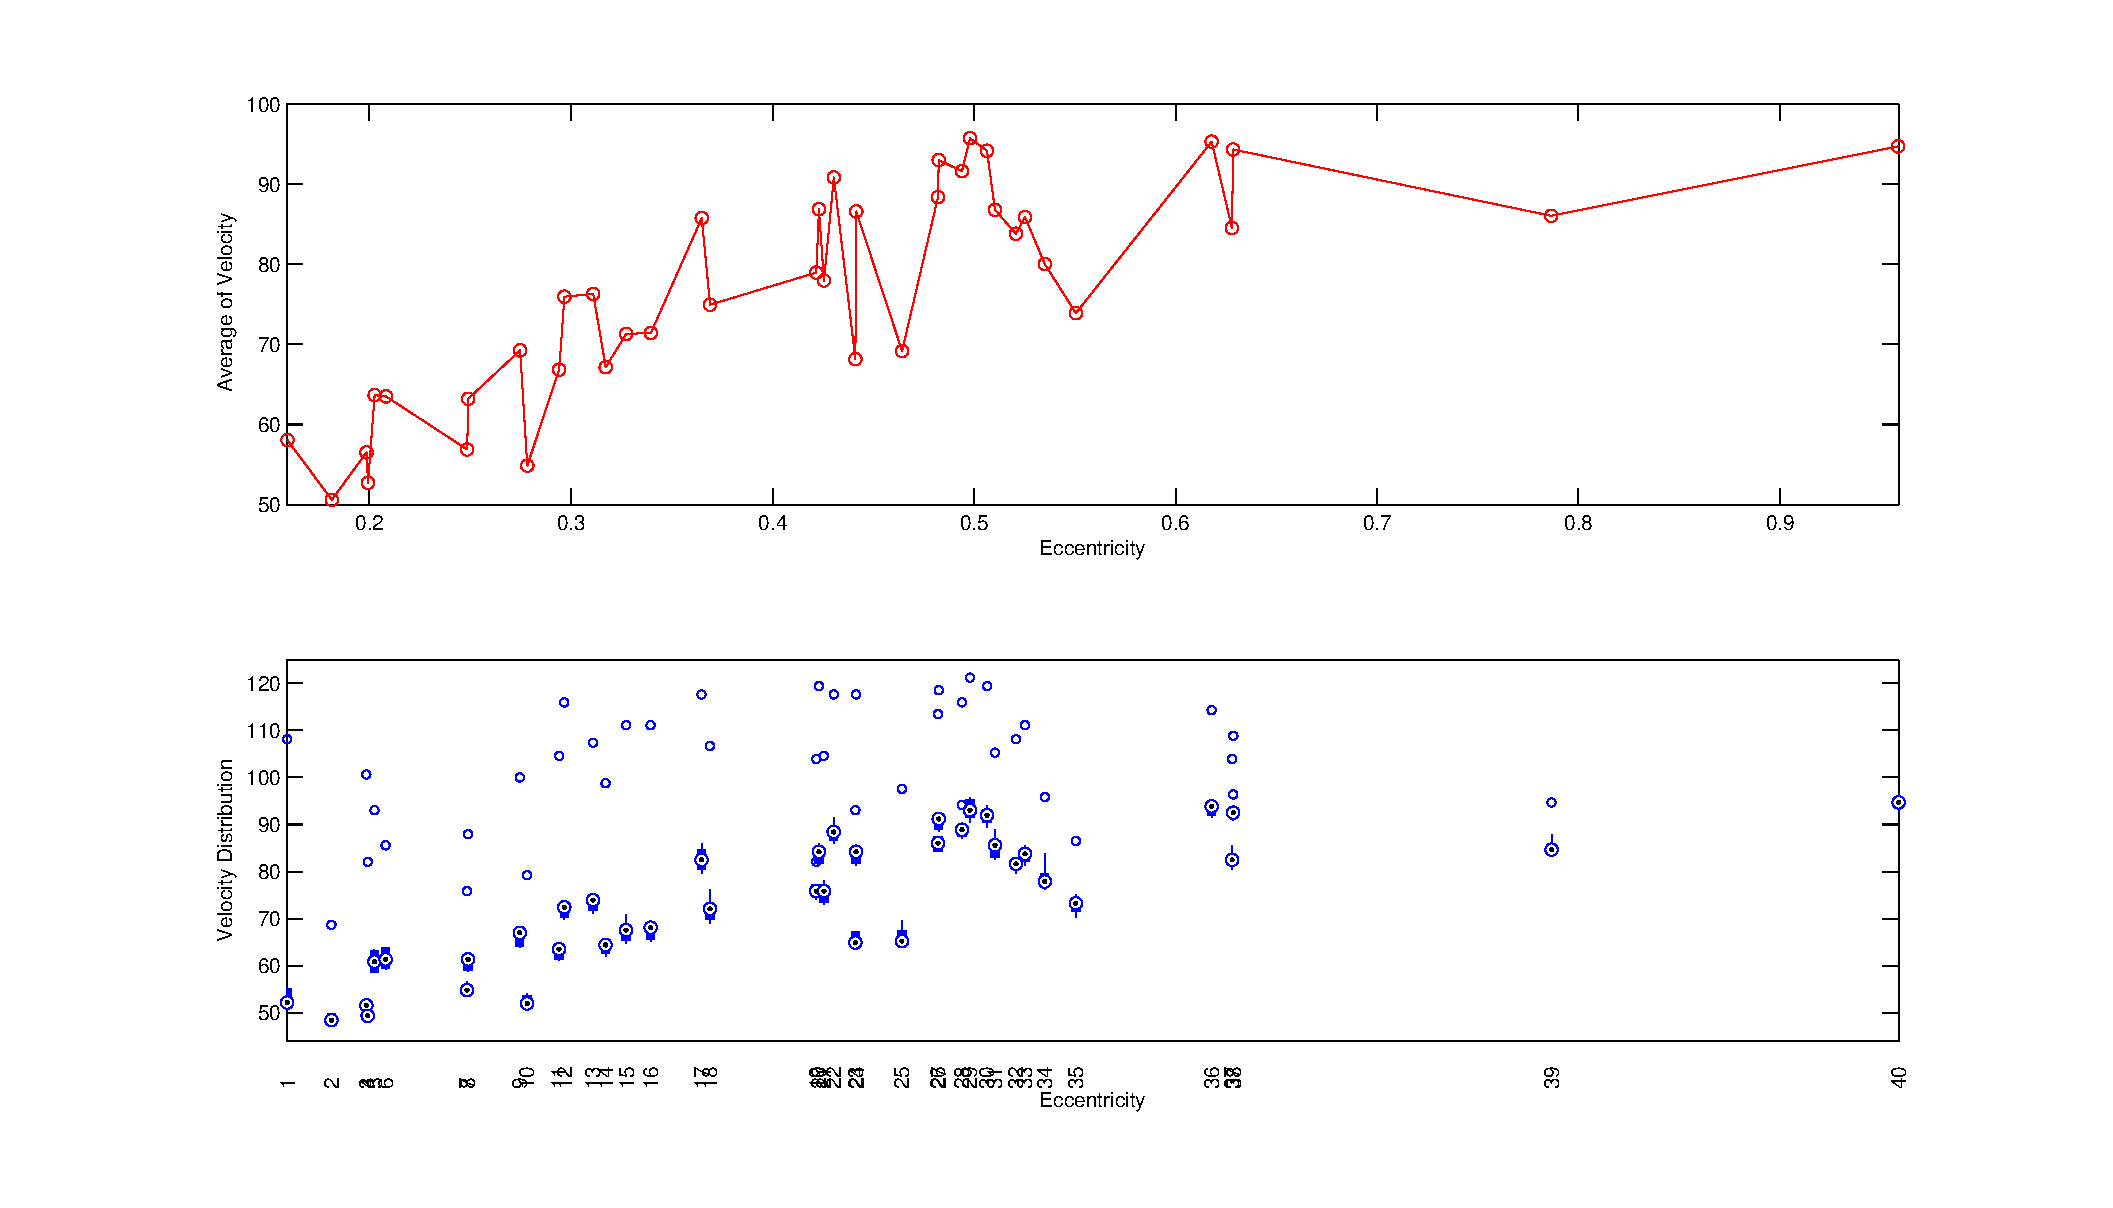
\includegraphics[width=500pt]{fig2.eps}
\caption{Ellipse eccentricity vs average velocity.  y-values were obtained by averaging over multiple drops for each shape.   }
\label{default}
\end{center}
\end{figure*}

\end{document}
